% !TEX root = ../MasterThesis_Onoe.tex
% 上記はただのコメントではなく親ファイルの場所を教えているので
% 消してしまうとファイルごとのタイプセットができなくなるので注意。
% 親ファイル名を変更したときはここも変更する。

\appendix 

\chapter{付録A} \label{sec:Appendix}
\section{LCIO parameter}
記入予定です。
\begin{figure}[H]
	\begin{center}
 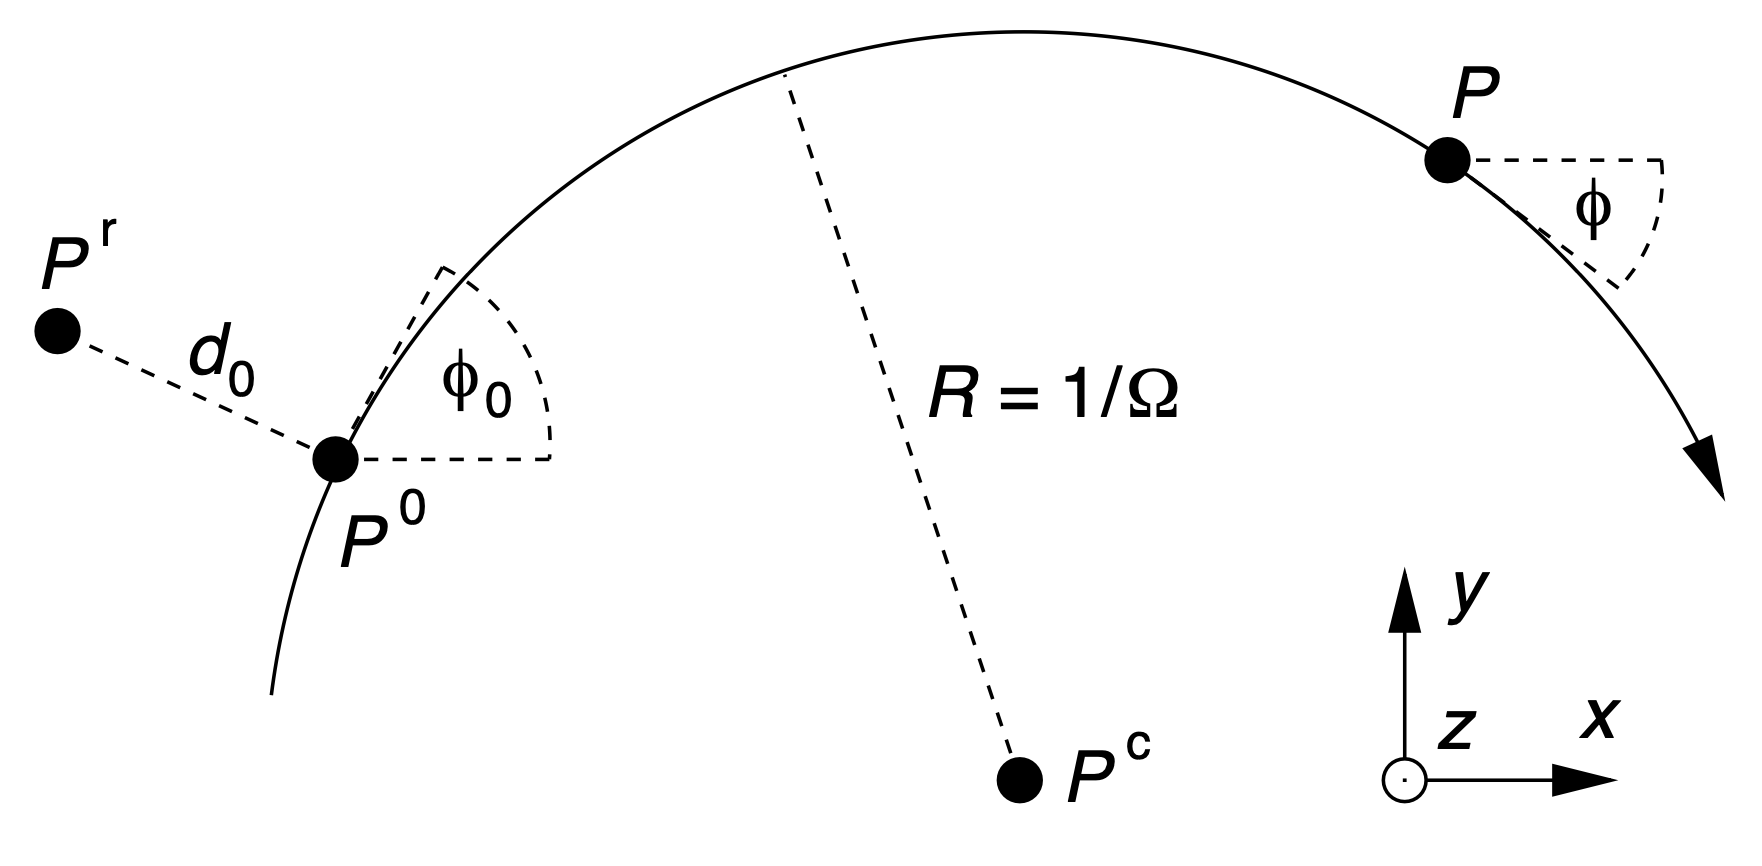
\includegraphics[keepaspectratio, scale=0.4]
 	{Figure/Appendix/xy.png}
 		\caption{xy平面}
 		\label{xy}
	\end{center}
\end{figure}
\begin{figure}[H]
	\begin{center}
 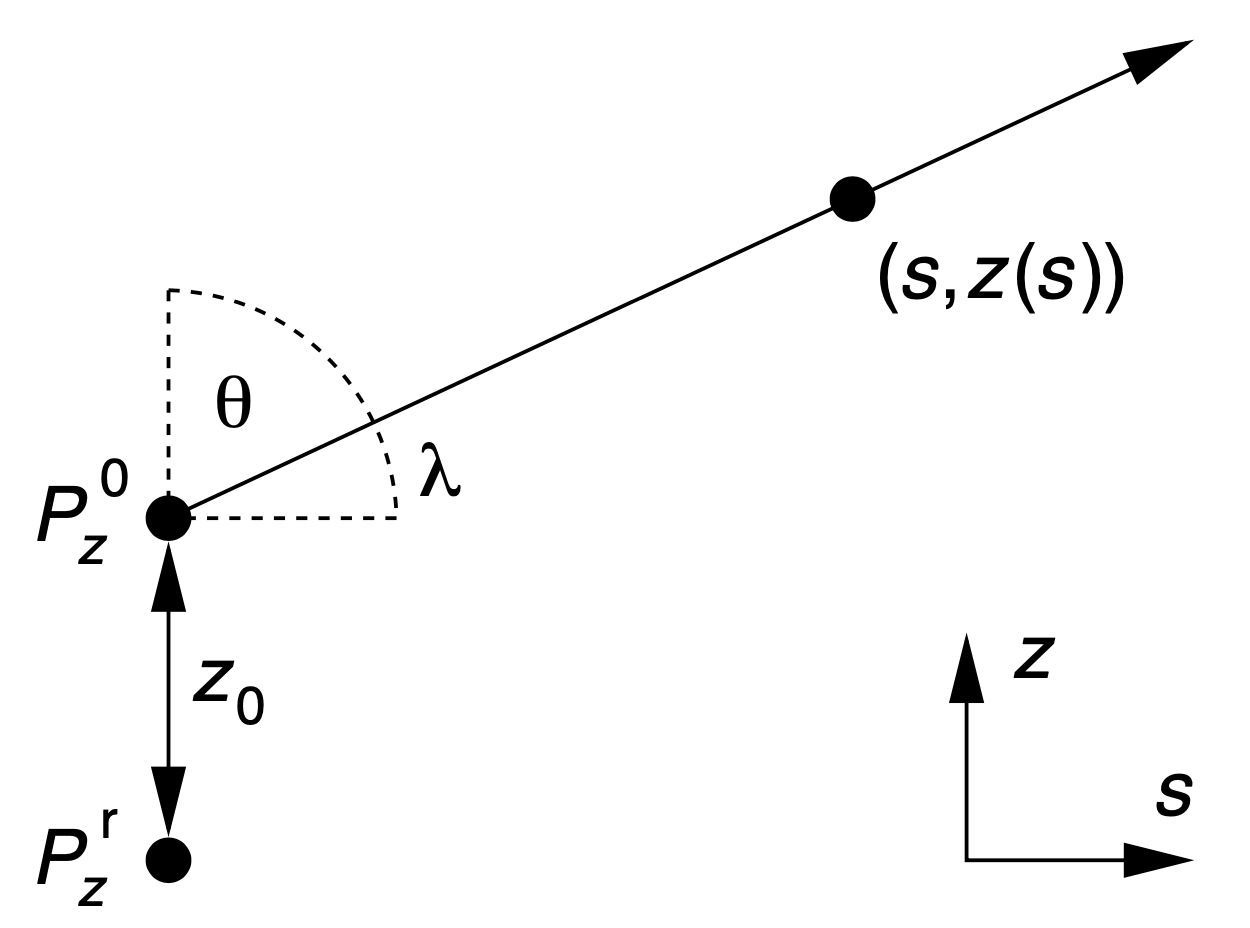
\includegraphics[keepaspectratio, scale=0.4]
 	{Figure/Appendix/sz.png}
 		\caption{sz平面}
 		\label{sz}
	\end{center}
\end{figure}
